\documentclass[a4paper,10pt, spanish]{article}

\usepackage{graphicx}
\usepackage{listings}
\usepackage[final]{pdfpages}
\usepackage[spanish]{babel}
\usepackage[utf8]{inputenc}
\usepackage[export]{adjustbox}
\usepackage{mips}

\lstset{
language=C,
tabsize=2,
  basicstyle=\small\ttfamily,
  columns=fullflexible,
  frame=single,
  breaklines=true,
  resetmargins=true
}

\title{
            \large{Organización de Computadoras} \\
            \textbf{Trabajo Práctico 1} \\
            \textbf{Implementación en MIPS Assembly} \\
            \bigskip
            
\includegraphics[max height=100pt,max width=100pt]{./UBA.png} \\
}

\author{	Nicolás Ledesma, \textit{Padrón Nro. 93.118}                        \\
            \texttt{ nicolas.angel.ledesma@gmail.com }                           \\[2.5ex]
            Jonathan Moguilevsky, \textit{Padrón Nro. 95.516}                   \\
            \texttt{ jmoguilevsky@gmail.com }                                   \\[2.5ex]
            Leonardo Riego, \textit{Padrón Nro. 94.104}                 \\
            \texttt{ riegoleonardo@hotmail.com }                                          \\[2.5ex]
            \normalsize{2do. Cuatrimestre de 2019}                              \\
            \normalsize{66.20 Org. de Computadoras
                $-$ Práctica: Santi, Pérez Masci, Natale }                      \\
            \normalsize{Facultad de Ingeniería, Universidad de Buenos Aires}    \\
       }
\date{}

\begin{document}

\maketitle

\thispagestyle{empty}   % quita el número en la primer página


\begin{abstract}
Este trabajo práctico grupal tiene como objetivo principal.
\end{abstract}

\pagebreak

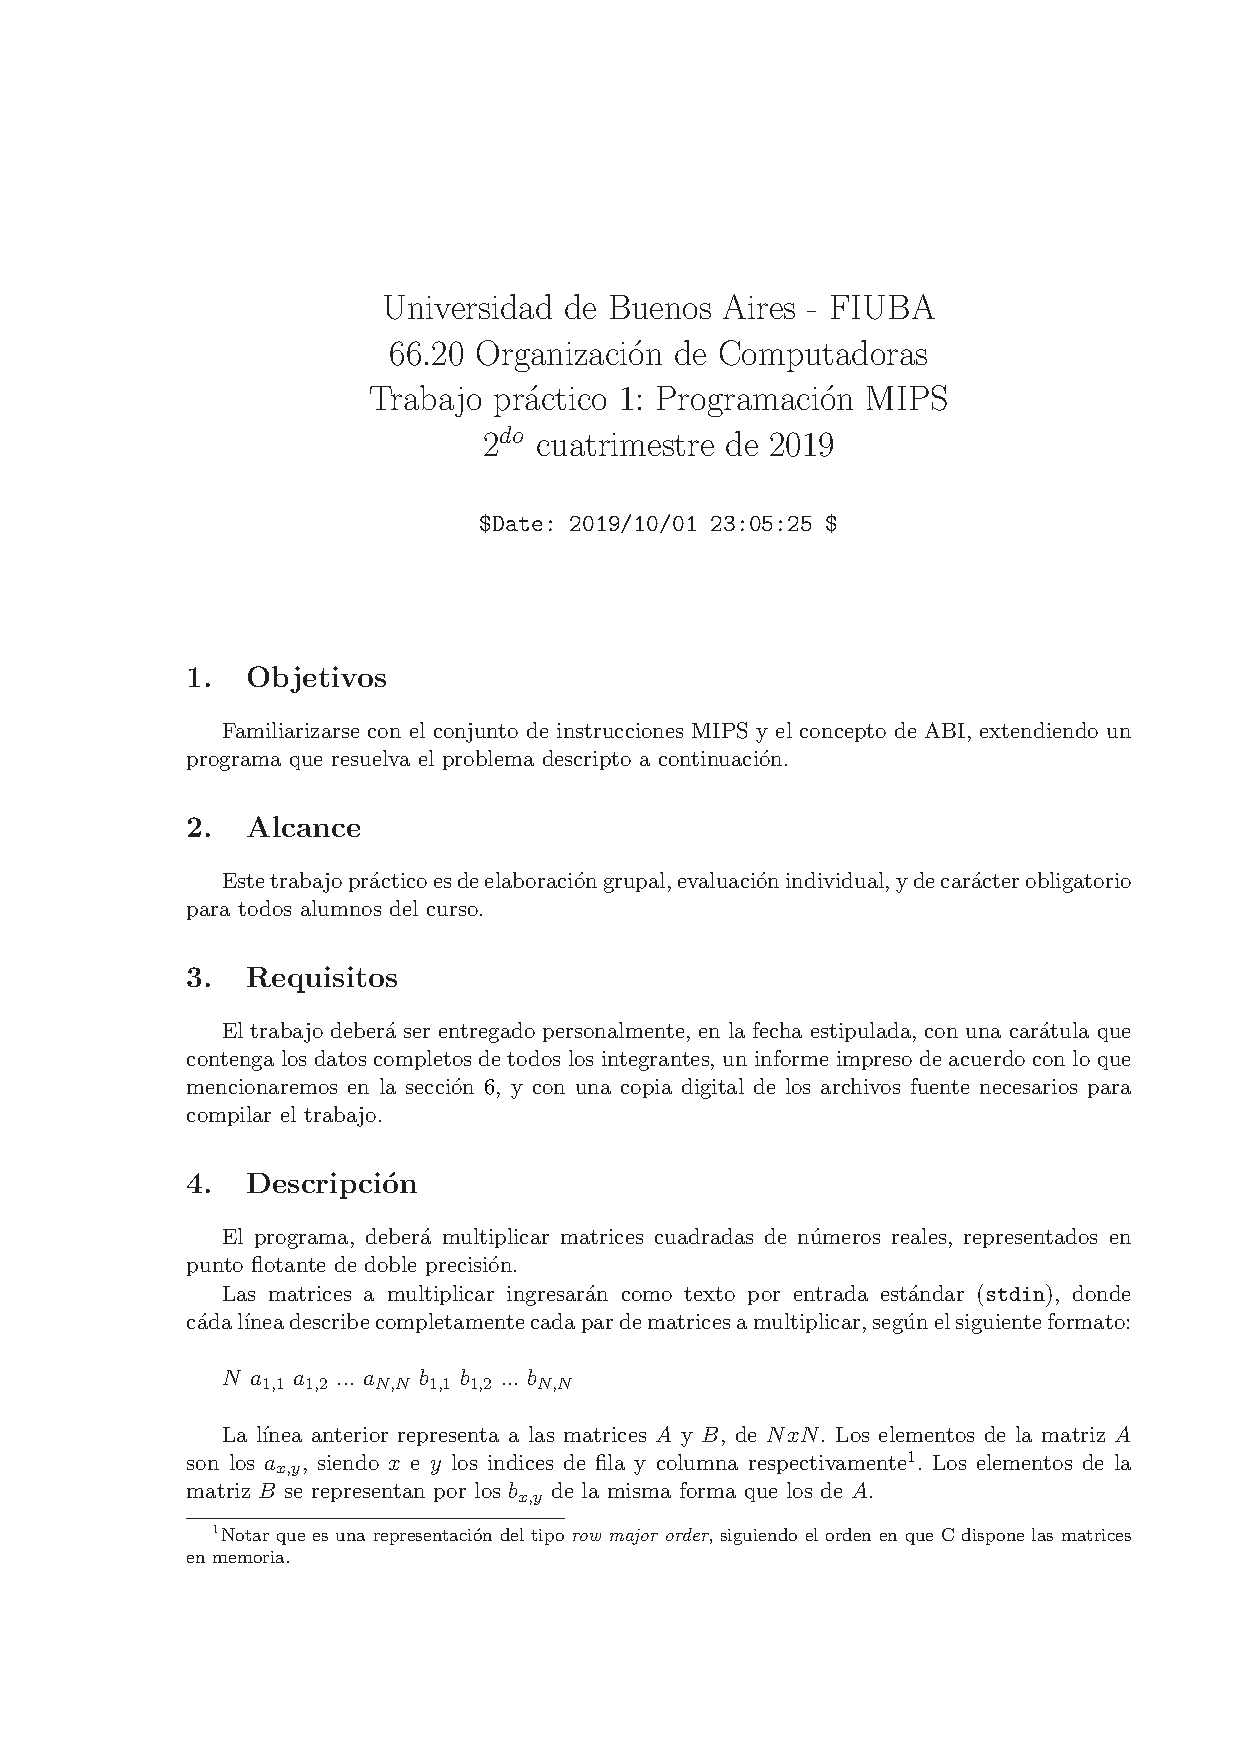
\includepdf[
    trim=20mm 30mm 10mm 25mm, clip,
    pages=1,
    frame,
    scale=.65,
    pagecommand=\section{Enunciado}
 ]{./tp1-2019-2q.pdf}
\includepdf[
    trim=20mm 30mm 10mm 25mm, clip,
    pages=2-,
    frame,
    scale=.65,
    pagecommand={}
 ]{./tp1-2019-2q.pdf}

\section{Solución}

\subsection{Diseño}
Se conservaron del código escrito para el anterior trabajo práctico las funciones dedicadas a procesamiento que se dedica a la lectura y procesamiento de las matrices ingresadas para su utilización, desde leer el input ingresado hasta formatearlo como es necesario, y la presentación impresión de menús y mensajes de error respectivamente.

Por otra parte, se implementaron en lenguaje assembly de MIPS las funciones \textbf{matrix\_multiply} y \textbf{create\_matrix}

\subsubsection{matrix\_multiply}
Función encargada del cálculo del producto de las matrices ingresadas. \\
    \lstinline{Stack frame} \\
            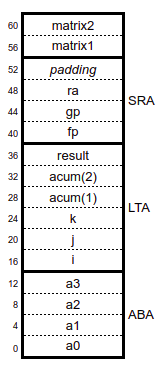
\includegraphics[max height=100pt,max width=100pt]{./stack_matrix_multiply.png}
            \begin{itemize}
                \item \lstinline{SRA}
                Se guardaron los registros gp, fp y ra en este área, con 4 bytes de padding para que quede alineada a 8 bytes como dicta la ABI
                \item \lstinline{LTA}
                Se reservaron espacios de memoria para las variables i, j y k que son los contadores utilizados en los distintos loops, 8 bytes para la variable acum utilizada para guardar los resultados parciales, y result que es utilizado como puntero a la estructura que guarda el resultado final.
            \end{itemize}

           Además, se definieron las constantes STACK\_SIZE(tamaño del stack), OFFSET\_RA, OFFSET\_FP y OFFSET\_GP para los offsets de las posiciones de memoria donde se guardaran los registros ra, fp y gp respectivamente

\subsubsection{create\_matrix}
    Función encargada de reservar memoria para una matriz con las dimensiones recibidas por parametro \\
    \lstinline{Stack frame} \\
            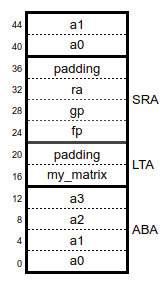
\includegraphics[max height=100pt,max width=100pt]{./stack_create_matrix.png}
            \begin{itemize}
                \item \lstinline{SRA}
                Se guardaron los registros gp, fp y ra en este área, con 4 bytes de padding para que quede alineada a 8 bytes como dicta la ABI
                \item \lstinline{LTA}
                Se reserva una posicion en el stack donde se guardará la dirección de memoria de la matriz creada
            \end{itemize}
     Además, se definieron las siguientes constantes:
        \begin{itemize}
            \item \lstinline{STACK_SIZE_CREATE_MATRIX:} tamaño stack
            \item \lstinline{OFFSET_RA_CREATE_MATRIX:} offset ra
            \item \lstinline{OFFSET_GP_CREATE_MATRIX:} offset gp
            \item \lstinline{OFFSET_FP_CREATE_MATRIX:} offset fp
            \item \lstinline{OFFSET_MY_MATRIX_CREATE_MATRIX:} offset variable my\_matrix
            \item \lstinline{A0_CALLEE_CREATE_MATRIX:} offset primer registro ABA
            \item \lstinline{A0_CALLER_CREATE_MATRIX:} offset primer argumento de la función
            \item \lstinline{A1_CALLER_CREATE_MATRIX:} offset segundo agurmento de la funcion
        \end{itemize}


\subsection{Código}

\lstinputlisting{../dynamic.c}
\lstinputlisting{../matrix_multiply.S}

\lstset{
  language=bash,
  basicstyle=\small\ttfamily
}

\subsection{Compilación del programa}
Para compilar el programa se utiliza el makefile desde el directorio donde se descomprimió el entregable:
\begin{lstlisting}
$ make clean
$ make all
gcc -Wall -c dynamic.c
gcc -o dynamic dynamic.o

\end{lstlisting}

\section{Pruebas}

\subsubsection{Ejecución}

Para la ejecución de las pruebas generamos un script llamado \lstinline{run_tests.sh} que se encarga de, para cada caso generado, ejecutar el programa y escribit el output en un archivo.
Finalmente, se comparan los outputs contra archivos que contienen los resultados esperados, en la carpeta \lstinline{results/}.

\subsection{Casos de prueba}

Para probar nuestro programa generamos una serie de casos de prueba:

\begin{itemize}
  \item \lstinline{big_matrix_ints.txt:} Matriz de 100x100 con valores enteros
	\item \lstinline{big_matrix_doubles.txt:} Matriz de 100x100 con valores de punto flotante
  \item \lstinline{exponential_doubles_matrix.txt:} Matriz pequeña con valores de punto flotante en notación exponencial.
  \item \lstinline{invalid_input.txt:} Prueba con input invalido.
  \item \lstinline{simple_multiline.txt:} Prueba de input con varias líneas.
  \item \lstinline{single_line.txt:} Prueba simple de una sola línea.
  \item \lstinline{small_double_matrix.txt:} Prueba simple de una matriz 3x3 de doubles.
  \item \lstinline{small_int_matrix.txt:} Prueba simple de una matriz 3x3 de integers.
\end{itemize}

La ejecución de los casos se realiza de la siguiente manera:

\begin{lstlisting}
$ ./run_tests.sh
\end{lstlisting}

Este script de ejecución valida también la impresión del menú y de la versión del programa.

\section{Conclusiones}

Como conclusión se puede ver en principio como al trabajar un programa a nivel de assembly, y necesitar uno crear el stack frame, se tiene pleno control(sin olvidar respetar la ABI) y conocimiento del uso de la memoria principal del programa que se cree.

Se observa a su vez que las gestión de recursos de la máquina es absoluta, tanto en el uso de memoria como de los registros del procesador, pero en detrimento de la legibilidad y de perder herramientas para visualizar errores que van surgiendo durante el desarrollo.

\end{document}
